\section{Vectors}

\begin{frame}
	\frametitle{Vectors and spatential interpretation}
	\begin{block}{Properties of a vector}
		There are 3 properties of a vector $\overrightarrow{x}$:
		\begin{itemize}
			\item magnitude
			\item direction
			\item startpoint
		\end{itemize}
		{\bf with respect to} a referention vector $\overrightarrow{0}$
	\end{block}
\end{frame}

\begin{frame}
	\begin{block}{Multiplication scalar and vector}
		r $\epsilon$ $\mathbb{R}$ (r $\epsilon$ $\mathbb{C}$ is possible, but hasn't a fysical representation)
		\begin{itemize}
			\item $|r|<1$: shorten
			\item $|r|>1$: increase
			\item $r<0$: reverse the direction
		\end{itemize}
	\end{block}
	\begin{block}{Addition of vectors}
		Parallellogramrule:

		\begin{figure}
			\centering
			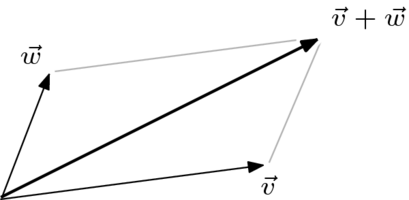
\includegraphics[width=0.4\linewidth]{optelling}
		\end{figure}
	\end{block} 
\end{frame}

\begin{frame}
	\frametitle{vectorspace}
	\begin{block}{First condition}
		A vectorspace V over a body L (set of operators) is a set of vectors that satisfy:\\
		1. A vectorsum is defined: $VxV\rightarrow V:(\overrightarrow{x},\overrightarrow{y})\rightarrow\overrightarrow{x}+\overrightarrow{y}$\\
		 \hspace{1.5 cm}$\overrightarrow{x}$, $\overrightarrow{y}$, $\overrightarrow{z}$ $\epsilon$ V
		\begin{description}
			\item[a)] $\overrightarrow{x}+\overrightarrow{y}$ $\epsilon$ V
			\item[b)] $\overrightarrow{x}+(\overrightarrow{y}+\overrightarrow{z})=(\overrightarrow{x}+\overrightarrow{y})+\overrightarrow{z}$
			\item[c)] $\exists!\overrightarrow{0}: \overrightarrow{x}+\overrightarrow{0}=\overrightarrow{0}+\overrightarrow{x}=\overrightarrow{x}$
			\item[d)] $\forall \overrightarrow{x}, \exists (-\overrightarrow{x}):\overrightarrow{x}+(-\overrightarrow{x})=(-\overrightarrow{x})+\overrightarrow{x}=0$
			\item[e)] $\overrightarrow{x}+\overrightarrow{y}=\overrightarrow{y}+\overrightarrow{x}$
		\end{description}
	\end{block}
\end{frame}

\begin{frame}
	\frametitle{vectorspace}
	\begin{block}{Second condition}
		2. A outside law is defined:$LxV\rightarrow V:(a,\overrightarrow{x})\rightarrow a\overrightarrow{x}$\\
		\hspace{1.5 cm}$\overrightarrow{x}$, $\overrightarrow{y}$ $\epsilon$ V\\
		\hspace{1.5 cm}a,b $\epsilon$ L
		\begin{description}
			\item[a)] $1\overrightarrow{x}=\overrightarrow{x}$
			\item[b)] $a(b\overrightarrow{x})=(ab)\overrightarrow{x}$
			\item[c)] $(a+b)\overrightarrow{x}=a\overrightarrow{x}+b\overrightarrow{x}$
			\item[d)] $a(\overrightarrow{x}+\overrightarrow{y})=a\overrightarrow{x}+a\overrightarrow{y}$
		\end{description}
	\end{block} 
\end{frame}

\begin{frame}
	\frametitle{Numberspaces of n-couples}
	\begin{block}{Defenition}
		This is the set of all n-couples like 
		$\begin{bmatrix}
			\overrightarrow{x_1}\\
			\overrightarrow{x_2}\\
			.\\
			.\\
			\overrightarrow{x_n}
		\end{bmatrix}$ with $x_i$ $\epsilon$ $\mathbb{R}$ or $x_i$ $\epsilon$ $\mathbb{C}$.\\
		This set together with the operator set $\mathbb{R}$ or $\mathbb{C}$ is a vectorspace.
	\end{block}
\end{frame}
		
\begin{frame}
	\frametitle{Subspaces}
	\begin{block}{Defenition}
		$V_1$ is a supspace of vectorspace V if:\\ 
		\begin{enumerate}
			\item $V_1 \subset$ V
			\item With the same in- and outside law as V, is $V_1$ a vectorspace
		\end{enumerate}
	\end{block}
	\begin{block}{Properties}
		\begin{enumerate}
			\item $\overrightarrow{0}$ $\epsilon$ every subspace
			\item The intersection of two spaces is always a subspace
			\item Given: p vectors $x_1,x_2,...,x_p$ $\epsilon$ V.\\
			The set vectors $a_1x_1+a_2x_2+...+a_nx_n$ with $a_i$ $\epsilon$ $\mathbb{R}$ is a subspace of V.
		\end{enumerate}
	\end{block}
\end{frame}

\begin{frame}
	\frametitle{Linear independance, basis, dimensions}
	\begin{block}{Defenition independance}
		Given: p vectors $\overrightarrow{x_1},\overrightarrow{x_2},...,\overrightarrow{x_p}$ $\epsilon$ V.\\
		Construct the nullvector as a linear combination of those vectors (i.e. search the operators (numbers) $a_1,a_2,...,a_p$ to form $a_1\overrightarrow{x_1}+a_2\overrightarrow{x_2}+...+a_n\overrightarrow{x_n}=\overrightarrow{0}$).\\
		If the nullvector only can created by $a_1=a_2=...=a_p=0$, then are the vectors $\overrightarrow{x_1},\overrightarrow{x_2},...,\overrightarrow{x_p}$ {\bf linear independant}.
	\end{block}
\end{frame}

\begin{frame}
	\frametitle{Linear independance, basis, dimensions}
	\begin{block}{Properties}
		\begin{enumerate}
			\item If the vectors $\overrightarrow{x_1},\overrightarrow{x_2},...,\overrightarrow{x_p}$ are linear independent, then can't none of them be writed as a linear combination of the other p-1 vectors.
			\item If the nullvector is one of the p vectors, then is the set $\overrightarrow{x_1},\overrightarrow{x_2},...,\overrightarrow{x_p}$ linear dependant (if $\overrightarrow{x_1}=0$ then is $a_1\overrightarrow{x_1}+a_2\overrightarrow{x_2}+...+a_n\overrightarrow{x_n}=0$ with $a_1\neq0$ and $a_2,a_3,...a_p=0$).
			\item Basis and dimension: p linear independant vectors $\overrightarrow{x_1},\overrightarrow{x_2},...,\overrightarrow{x_p}$ generate a vectrospace $V^p$. Every vector in $V^p$ can be writed {\bf in only one way} as a linear combination of the p linear independant vectors $\overrightarrow{x_1},\overrightarrow{x_2},...,\overrightarrow{x_p}$ using operators $a_1,a_2,...,a_p$.
		\end{enumerate}
	\end{block}
\end{frame}

\begin{frame}
	\frametitle{Linear independance, basis, dimensions}
	\begin{block}{Basis, dimension}
		Given: $\overrightarrow{v}=a_1\overrightarrow{x_1}+a_2\overrightarrow{x_2}+...+a_p\overrightarrow{x_p}$.\\
		The set operators $a_1,a_2,...,a_p$ are called the {\bf coordinates} of the vector $\overrightarrow{v}$ relative to the set vectors $\overrightarrow{x_1},\overrightarrow{x_2},...,\overrightarrow{x_p}$. This set vectors is a {\bf basis} of vectorspace $V^p$, with {\bf dimension} p.
	\end{block}
\end{frame}

\begin{frame}
	\frametitle{Linear independance, basis, dimensions}
	\begin{block}{Example}
		Given: $\overrightarrow{x_1}=\begin{bmatrix} 1\\0\\0\end{bmatrix}, \overrightarrow{x_2}=\begin{bmatrix} 0\\1\\0\end{bmatrix}, \overrightarrow{x_3}=\begin{bmatrix} 0\\0\\1\end{bmatrix}$\\
		The set \big\{$\overrightarrow{x_1},\overrightarrow{x_2},\overrightarrow{x_3}$\big\} is a linear independant combination. There doesn't exist numbers $a_1\neq0$, $a_2\neq0$, $a_3\neq0$ such that $a_1\overrightarrow{x_1}+a_2\overrightarrow{x_2}+a_n\overrightarrow{x_3}=0$. The set of all vectors $\overrightarrow{y}= a_1\overrightarrow{x_1}+ a_2\overrightarrow{x_2}+ a_n\overrightarrow{x_3}$ is the three dimensional vectrospace $V^3$.\\
		If $\overrightarrow{y}=\begin{bmatrix} 3\\2\\1\end{bmatrix}$. Then is $3\overrightarrow{x_1}+2\overrightarrow{x_2}+\overrightarrow{x_3}$ the only way to write $\overrightarrow{y}$ as a linear combination of $\overrightarrow{x_1},\overrightarrow{x_2},\overrightarrow{x_3}$.
	\end{block}
\end{frame}

\begin{frame}
	\frametitle{Linear independance, basis, dimensions}
	\begin{block}{Example}
		The set of vectors $\overrightarrow{y}=a_1\overrightarrow{x_1}+a_2\overrightarrow{x_2}$ is a {\bf two dimensional} subspace $V^2$.\\
		The vectors in this subspace are: $\overrightarrow{y}=\begin{bmatrix} y_1\\y_2\\y_3\end{bmatrix}=a_1\begin{bmatrix} 1\\0\\0\end{bmatrix}+ a_2\begin{bmatrix} 0\\1\\0\end{bmatrix}=\begin{bmatrix} a_1\\a_2\\0\end{bmatrix}$.
	\end{block}
	\begin{block}{Important difference}
		\begin{itemize}
			\item All vectors of $V^2$ have \textbf{3} coordinates.
			\item The dimension of the subspace $V^2$ is \textbf{2}.
		\end{itemize}
	\end{block}
\end{frame}

\begin{frame}
	\frametitle{Linear independance, basis, dimensions}
	\begin{block}{Convention of notation}
		Given: a n-dimensional vectorspace $V^n$.\\
		The elements of this vectorspace are the elements: $\overrightarrow{x},\overrightarrow{y},..$. If we choose $\overrightarrow{e_1},\overrightarrow{e_2},...,\overrightarrow{e_n}$ as a basis of $V^n$. Then we can write every vector of $V^n$ as a linear combination of those basis vectors in only one way: $\overrightarrow{x}=x_1\overrightarrow{e_1}+x_2\overrightarrow{e_2}+ ...+x_n\overrightarrow{e_n}$. The numbers $x_i$ are the coordinates of vector $\overrightarrow{x}$ relative to the basis $\overrightarrow{e_1},\overrightarrow{e_2},..., \overrightarrow{e_n}$.\vspace{5mm}
		Between the vectorspace of dimension n and the number space of dimension n exists a isomorphism.	
	\end{block}
\end{frame}

\begin{frame}
	\frametitle{Linear independance, basis, dimensions}
	\begin{block}{Vectorspace $V^p$}
		Given: a p-dimensional vectorspace $V^p$ where the vectors are n-couples (with $n\geq p$).
		\begin{enumerate}
			\item In $V^p$ you can choose a basis with p linear independant vectors.
			\item Every vector $\overrightarrow{x}$ $\epsilon$ $V^p$ can be writed in only one way as a linear combination of the p basis vectors using coordinates.
		\end{enumerate}	
	\end{block}
	\begin{block}{Example 1}
		Given: n=5, p=2, $\overrightarrow{x_1}=\begin{bmatrix} 1\\0\\-1\\2\\5\end{bmatrix}, \overrightarrow{x_2}=\begin{bmatrix} 2\\-3\\1\\0\\0\end{bmatrix}$.\\
	\end{block}
\end{frame}

\begin{frame}
	\frametitle{Linear independance, basis, dimensions}
	\begin{block}{Example 1}
		The vectors $\overrightarrow{x_1}$ and $\overrightarrow{x_2}$ are linear independant, so they span a two dimensional subspace: $\overrightarrow{y}=a_1\overrightarrow{x_1}+a_2\overrightarrow{x_2}$ with $a_1, a_2$ $\epsilon$ $\mathbb{R}$.\\
		The coordinates of the vector $y_1=\begin{bmatrix} 5\\-6\\1\\2\\5\end{bmatrix}$, relative to the basis \big\{$\overrightarrow{x_1},\overrightarrow{x_2}$\big\}, are $a_1=1$ and $a_2=2$.
	\end{block}
\end{frame}

\begin{frame}
	\frametitle{Linear independance, basis, dimensions}
	\begin{block}{Example 1}
		The vector $\overrightarrow{y_2}=\begin{bmatrix} 5\\-7\\1\\2\\5\end{bmatrix}$ can't be writen as a linear combination of the vectors $\overrightarrow{x_1}$ and $\overrightarrow{x_2}$. So $y_2$ doesn't belong to the subspace spanned by $\overrightarrow{x_1}$ and $\overrightarrow{x_2}$.\\
		This implies that $\overrightarrow{y_2}$ is linear independant of $\overrightarrow{x_1}$ and $\overrightarrow{x_2}$. Thus the subspace spanned by $\overrightarrow{y_2}$, $\overrightarrow{x_1}$ and $\overrightarrow{x_2}$ is a 3 dimensional subspace.
	\end{block}
\end{frame}

\begin{frame}
	\frametitle{Linear independance, basis, dimensions}
	\begin{block}{In general}
		When the set vectors $\overrightarrow{x_1},\overrightarrow{x_2},..., \overrightarrow{x_p}$ is linear independant, then lays $\overrightarrow{x_i}$ not totally in the subspace spanned by the vectors $\overrightarrow{x_1},..., \overrightarrow{x}_{i-1}, \overrightarrow{x}_{i+1},...,\overrightarrow{x_p}$.\\
		The vector $\overrightarrow{x_i}$ can be writen as a sum of 2 components: $\overrightarrow{x}_{i\alpha}$ and $\overrightarrow{x}_{i\beta}$.
		\begin{enumerate}
			\item $\overrightarrow{x}_{i\alpha}$ $\epsilon$ subspace spanned by $\overrightarrow{x_1},..., \overrightarrow{x}_{i-1}, \overrightarrow{x}_{i+1},...,\overrightarrow{x_p}$.
			\item $\overrightarrow{x}_{i\beta}$ $\bot$ subspace spanned by $\overrightarrow{x_1},..., \overrightarrow{x}_{i-1}, \overrightarrow{x}_{i+1},...,\overrightarrow{x_p}$.
		\end{enumerate}
	\end{block}
\end{frame}

\begin{frame}
	\frametitle{Inproduct}
	\begin{block}{Defenition}
		The inproduct of two vectors $\overrightarrow{x}$ and $\overrightarrow{y}$ $\epsilon$ $E^n$ (n-couples) is defined as the image: $E^nxE^n\to\mathbb{R}:\{\overrightarrow{x},\overrightarrow{y}\}\to\overrightarrow{x}.\overrightarrow{y}$ $\epsilon$ $\mathbb{R}$. This image is:
		\begin{enumerate}
			\item Linear
			\item Symetric
			\item Positive definite
		\end{enumerate}
	\end{block}
	\begin{block}{applied}
		$\forall \overrightarrow{x},\overrightarrow{y}$ $\epsilon$ $E^n$:
		\begin{enumerate}
			\item Bilinear: $(\overrightarrow{x}+\overrightarrow{v}).\overrightarrow{y}=\overrightarrow{x}\overrightarrow{y}+\overrightarrow{v}\overrightarrow{y}$
			\item
			\item
		\end{enumerate}
	\end{block} 
\end{frame}


	\subsection{Inproduct (scalair product)}
	\subsection{Gram-Schmidt orthogonalisation}
	\subsection{Complementary subspace}
	
	




